\documentclass[11pt,a4paper]{report}
\usepackage{ucs}
\usepackage[utf8]{inputenc}
\usepackage[T1]{fontenc}
\usepackage{amsmath}
\usepackage{amsfonts}
\usepackage{amssymb}
\usepackage{graphicx}
\usepackage[ngerman]{babel}

\usepackage{hyperref}


\title{Abschlussbericht zum Projekt LVS-IR-Taubenstein}
\author{Lea Vanheyden, Zorana Spasojevic, Alexander Fogus}

\begin{document}
	
\maketitle
	
\tableofcontents

\listoffigures

\listoftables

\newpage

\chapter{Einleitung}

Als beliebtes Ziel für Touristen und Wintersportler besteht im Alpengebiet eine besondere Konfliktsituation zwischen Mensch- und Tierreich. Routen für Spaziergänger, Skifahrer und Skitourengänger grenzen oft direkt an Lebensräume von Wildtieren an und führen so zu Stress für das Wildtierreich. Die vom Deutschen Alpenverein (DAV) in Kooperation mit dem Freistaat Bayern auf den Weg gebrachte Kampagne "`Natürlich auf Tour"' soll für eine Sensibilisierung und Informationsgebung rund um das Thema Naturschutz dienen.

Neben der Aufklärung ist ein weiteres Ziel dabei, das Verhalten der menschlichen Besucher zu analysieren um daraus abzuleiten inwiefern man es womöglich steuern kann. In diesem Sinne untersuchte der DAV in Zusammenarbeit mit dem Departement für Geographie der LMU am Berg Taubenstein im Mangfallgebirge rund um den Spitzingsee in der Saison 18/19 und 19/20 den Anteil der Skitourengänger mit sogenannten LVS-Geräten. LVS-Gerät ist die Abkürzung für Lawinenverschüttetensuchgerät, mit Hilfe dieser Geräte können von Lawinen verschüttete Personen schnell gefunden werden. Personen, die ein LVS-Gerät dabeihaben, können mit diesem andere LVS-Geräte suchen und auch selbst gefunden werden.

Anhand der zur Verfügung gestellten Daten zur Saison 18/19 wird durch ein Modell der Anteil der Skitourengänger mit LVS-Gerät in Abhängigkeit von anderen Faktoren (wie z.B. Uhrzeit, Temperatur, Schneehöhe) analysiert .
Zudem wird untersucht, von welchen Einflussgrößen die Messfehler abhängen, welcher Art (Über-/Unterschätzung) sie sind und ob eine Struktur (mögl. Verteilung) vorliegt.
Unter Berücksichtigung der Erkenntnisse über die Messfehler werden Hypothesen aufgestellt, in welcher Form die Messfehler die geschätzten Abhängigkeiten beeinflussen.

Noch schreiben, was wir rausgefunden haben.

Quelle:
\url{https://de.wikipedia.org/wiki/Lawinenverschüttetensuchgerät}

\chapter{Datenbasis}

\section{Datengrundlage}

Um auf den Anteil der Skitourengängen, die ein LVS-Gerät bei sich hatten, schließen zu können, hat man Checkpoints aufgestellt. Für den Aufstieg am Taubenstein gibt es zwei Routen, eine Nord- und eine Südroute. Die genauen Lagen kann man Abbildung \ref{pic:checkpoints} entnehmen. An beiden Routen wurde jeweils ein Checkpoint aufgestellt, an dem vorbeigehende Besucher gemessen werden. Durch Infrarotmessung wird erfasst, ob ein Mensch am Checkpoint vorbeigeht. Außerdem werden LVS-Geräte, die auf Sendebetrieb geschaltet sind, erfasst. Für jede einzelne Checkpointmessung liegt das jeweilige Datum mit Uhrzeit vor und an welcher der zwei Routen (N oder S) sie erfasst wurde.

\begin{figure}[h]
\centering
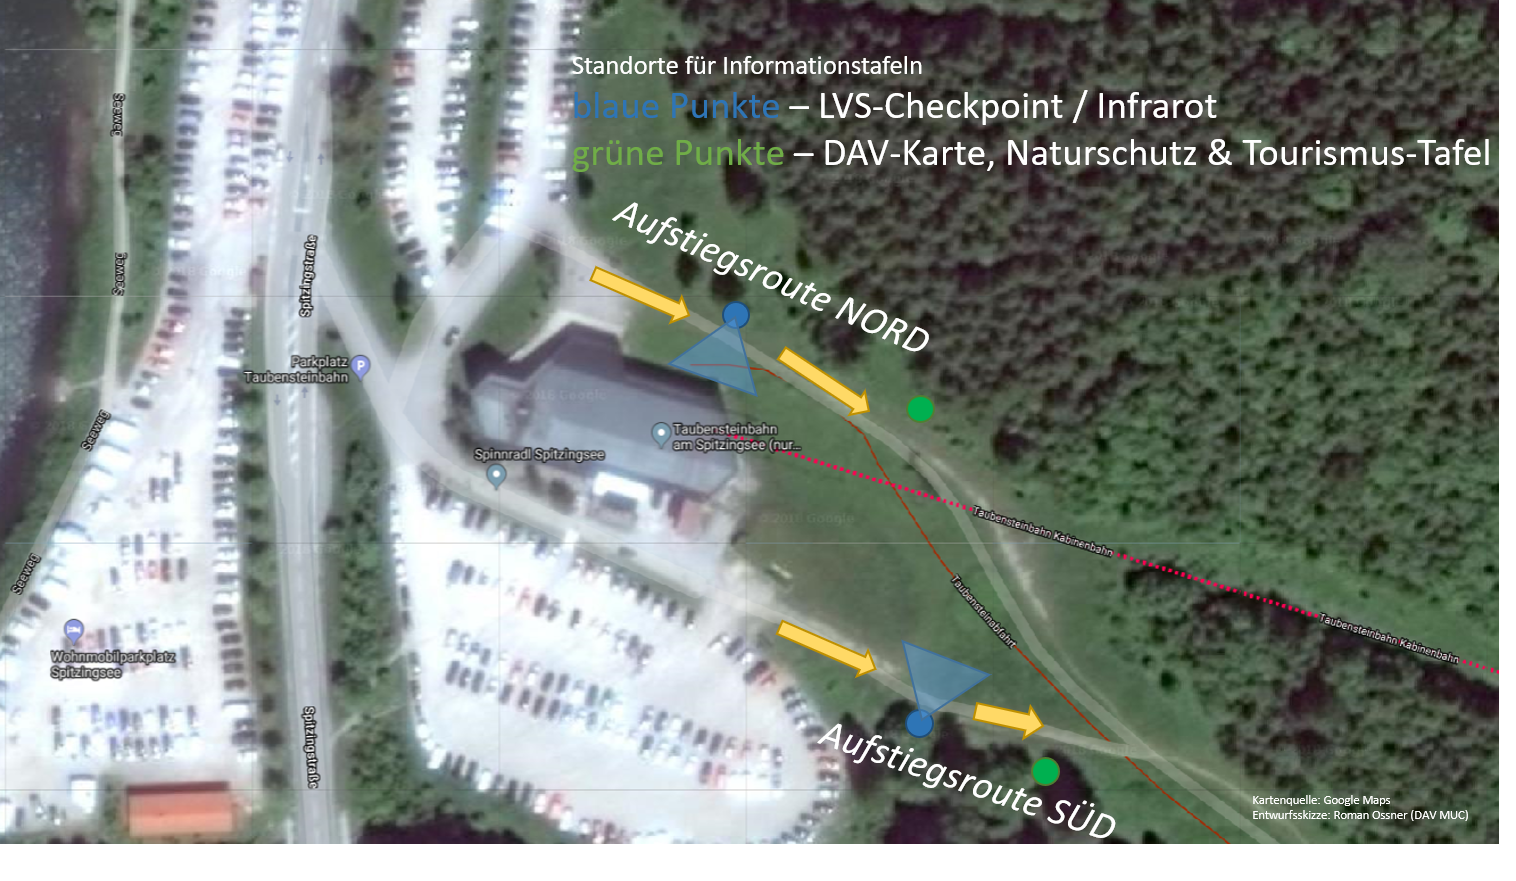
\includegraphics[scale=0.5]{Bilder/Checkpoints}
\caption[Checkpoints]{Satellitenbild, dass die Lage der zwei Routen und der Checkpoints verdeutlicht}
\label{pic:checkpoints}
\end{figure}

Für die erste Untersuchung benutzen wir vorerst nur diese automatisch erfassten Daten zur Saison 18/19. Der umfasste Zeitraum läuft dabei vom 21.12.2018 bis zum 13.04.2019. Anzumerken ist dabei, dass am 23.12. und 24.12. keine Messungen vorliegen, zudem werden Messungen vom 07.01. bis zum 15.01. außer Acht gelassen, da aufgrund von starkem Schneefall die Checkpoints bedeckt waren.

Zusätzlich zu diesen automatischen Messungen wurden manuell Gruppen von (?)Studenten/Mitarbeitern des Departments für Geographie(?) an bestimmten Tagen vor Ort eingesetzt, um durch Befragungen manuelle Daten zu gewinnen. Dabei wurde festgestellt, dass bei den durch die Checkpoints erhobenen Daten Messfehler vorliegen.

Quelle:
Folien vom Erstgespräch

Neben der Erfassung von Personen und LVS-Geräten liegen verschiedene weitere Daten vor.Für jeden Tag an dem gemessen wurde gibt es Information zu den Wetterbedingungen bzw. anderen möglichen Einflussvariablen. "`snowhight"' bemisst die Schneehöhe in cm. "`temperature"' ist die Temperatur des Tages um 12:00 mittags. "`solar\_radiation"' zeigt die Sonneneinstrahlung in $W/cm^2$. Außerdem sind die Lawinenwarnstufen des jeweiligen Tages angegeben. Es kann vorkommen, dass die Lawinenwarnstufe auf der Spitze des Berges eine andere ist als im Tal, deshalb gibt es zwei Variablen: "`avalanche\_report\_top"' und "`avalanche\_report\_down"'. Diese geben die Lawinenwarnstufe an der Spitze und am Fuß des Berges an. Obwohl es Stufen von 1 (niedrig) bis 5 (sehr hoch) gibt, war die in dem beobachteten Zeitraum höchste Stufe eine 4. An Tagen an denen die Stufen unterschiedlich waren wurde außerdem in "`avalanche\_report\_border"' der Höhenmeter angegeben, ab dem sich die Lawinengefahr unterscheidet. In "`avalanche\_report\_comment"' ist vermerkt, ob es sich dabei um eine Waldgrenze handelt. "`day"' gibt an, um welchen Tag der Woche es sich handelt und "`day\_weekday"', "`day\_weekend"' und "`holiday"' geben jeweils an, ob der Tag ein Tag unter der Woche oder am Wochenende war und ob er sich innerhalb einer Ferienzeit befunden hat.

\section{Datenaufbereitung}

Der erste Schritt besteht darin, die gegebenen Daten um weitere 
Bearbeitung der Daten durch uns:
(noch mehr schreiben)
sunnrise und sunset
"`count\_beacon"' und "`count\_infrared"' enthalten die Anzahl der gemessenen LVS-Geräte bzw. Infrarotmessungen pro Tag.
Umwandlung der Messungen zu Personendaten. Umstellung des Tages von 04:00 bis 04:00.
 Eine Übersicht über alle Variablen die verwendet wurden ist in Tabelle \ref{tab:var} zu finden.

\begin{table}
\caption{Übersicht aller benutzten Variablen mit kurzer Beschreibung}
\begin{tabular}{p{3cm}|p{5cm}|p{4cm}}
Name & Beschreibung & Werte \\
\hline
date & Datum & Datum vom 21.12.2018 bis zum 13.04.2019 \\
\hline
time & Uhrzeit(minutengenau) & Uhrzeit von 00:00 bis 24:00 \\
\hline
position & Route an der gemessen wurde & diskret (2 Ausprägungen): S,N \\
\hline
lvs & Hat die gemessene Person ein LVS-Gerät mitgeführt? & diskret (2 Auspr.): ja, nein \\
\hline
day & Wochentag & diskret (7 Auspr.): Montag, Dienstag,... \\
\hline
snowhight & Schneehöhe in cm (am Tag der Messung) & stetig: 16-212 \\
\hline
temperature & Temperatur in °C um 12:00 & stetig: (-7.9)-(9.7) \\
\hline
solar\_radiation & Sonneneinstrahlung in $W/cm^2$ & stetig: 14-792 \\
\hline
avalanche\_report & berechnete Lawinenwarnstufe & diskret (7 Auspr.): 1, 1.5, 2,... \\
\hline
holiday & Handelte es sich um einen Ferientag? & diskret (2 Auspr.): ja, nein \\
\hline
sunrise & Uhrzeit des Sonnenaufgangs & Uhrzeit von 05:57 bis 08:02 \\
\hline
sunset & Uhrzeit des Sonnenuntergangs & Uhrzeit von 16:22 bis 19:58 \\
\hline
day\_length & berechnete Länge des Tages (von Sonnenauf- bis Sonnenuntergang) & von 08:23 bis 13:28 h \\
\hline
\end{tabular}
\label{tab:var}
\end{table}

\section{Deskriptive Analyse}

Insgesamt 37593 Messungen an 114 Tagen

8468 Beacons, 29125 Infrareds (vor Umkodierung)

nach Umkodierung: 31574 Personen

8468 mit LVS-Gerät, 23106 ohne LVS-Gerät
pr
Die meisten Leute zwischen 09:00 und 18:00 unterwegs

--

Schneehöhe nimmt bis Mitte Januar stark zu und fällt ab Mitte Februar ab

Temperatur nimmt im Trend bus Mitte Januar ab und steigt danach
 
Sonnenstrahlung steigt bis März leicht und danach stark


---


Anteil schwankt in den ersten Wochen deutlich

generell viele Ausreißer, aber kein große Veränderung bei Schneehöhe, Temperatur und Sonneneinstrahlung

Anteile zur Mittagszeit geringer

mit steigender Lawinengefahr steigt die Anzahl

\chapter{Theorie und Beschreibung der verwendeten Modelle}

Logit-Modell?

Multivariates Logit-Modell?

gemischtes additives Modell?

Zeitreihenanalyse?
	
	
\end{document}